\documentclass[a4paper,12pt]{article}
\usepackage{cmap}
\usepackage{xfrac}
\usepackage[utf8]{inputenc}
\usepackage[T2A]{fontenc}
\usepackage[russian]{babel}
\usepackage{graphicx}
\usepackage{amsmath}
\usepackage{wrapfig}  % обтекание картинок текстом
\usepackage{minted}
\usepackage{tocloft}
\renewcommand{\cftsecleader}{\cftdotfill{\cftdotsep}}

\makeatletter
\renewcommand{\@biblabel}[1]{#1.} % Заменяем библиографию с квадратных скобок на точку:
\makeatother

\usepackage{geometry} % Меняем поля страницы
\geometry{left=2cm}% левое поле
\geometry{right=1.5cm}% правое поле
\geometry{top=1cm}% верхнее поле
\geometry{bottom=2cm}% нижнее поле

\renewcommand{\theenumi}{\arabic{enumi}}% Меняем везде перечисления на цифра.цифра
\renewcommand{\labelenumi}{\arabic{enumi}}% Меняем везде перечисления на цифра.цифра
\renewcommand{\theenumii}{.\arabic{enumii}}% Меняем везде перечисления на цифра.цифра
\renewcommand{\labelenumii}{\arabic{enumi}.\arabic{enumii}.}% Меняем везде перечисления на цифра.цифра
\renewcommand{\theenumiii}{.\arabic{enumiii}}% Меняем везде перечисления на цифра.цифра
\renewcommand{\labelenumiii}{\arabic{enumi}.\arabic{enumii}.\arabic{enumiii}.}% Меняем везде перечисления на цифра.цифра

\newcommand{\imgh}[3]{\begin{figure}[h]\center{\includegraphics[width=#1]{#2}}\caption{#3}\label{ris:#2}\end{figure}}



\begin{document}
\newpage

\begin{center}
    \large
    Московский авиационный институт \\
    национальный исследовательский университет\\
\end{center}

\vspace{8em}

\begin{center}
    \Large
    Факультет информационных технологий и прикладной математики\\
    Кафедра компьютерных методов в математическом моделировании сложных систем \\ 
\end{center}

\vspace{2em}

\begin{center}
    \textsc{\textbf{Курсовая работа по Эконометрике \linebreak на тему: \linebreak регрессионный анализ}}
\end{center}

\vspace{20em}



\newbox{\lbox}
\savebox{\lbox}{\hbox{Королев Егор Владимирович}}
\newlength{\maxl}
\setlength{\maxl}{\wd\lbox}
\hfill\parbox{11cm}{
    \hspace*{5cm}\hspace*{-5cm}Студент:\hfill\hbox to\maxl{Королев Егор Владимирович\hfill}\\
    \hspace*{5cm}\hspace*{-5cm}Преподаватель:\hfill\hbox to\maxl{Платонов Евгений Николаевич}\\
    \hspace*{5cm}\hspace*{-5cm}Группа:\hfill\hbox to\maxl{М8О-401Б-18}\\
}


\vspace{\fill}

\begin{center}
    Москва, 2021
\end{center}


\newpage
\tableofcontents
\newpage
\normalsize


\section{Задание}

\subsection{Теоретическая часть}
Написать эссе по Байесовской регрессии.



\subsection{Практическая часть}

\subsubsection{Модельная часть}

Смоделировать данные:
$$ X_k = f(h_k) + \varepsilon_k ,~~k=\overline{1,60}, $$
где $f(h) = 1.5h - 2 - \frac{1}{2h}$, $h\in [0.1;2]$, $\varepsilon_k$ -- независимый случайные величины с распределением $\mathcal{N}(0,\sigma^2)$.\\
Точки внутри носителя для h выбираются равномерно.\\
Смоделировать тестовую выборку объема 40, половина значений правее наблюдаемых значений, половина левее\\


\subsubsection{Метод наименьших квадратов}

Для регрессии вида:
$$ X_k = \theta_0 + \theta_1 h_k + \varepsilon_k, k=\overline{1,60} $$

\begin{enumerate}
    \item Найти МНК-оценки неизвестных параметров;
    \item построить график, на котором отобразить наблюдения, исходную функцию и линию регрессии;
    \item вычислить коэффициент детерминации и найти оценку ковариационной матрицы МНК-оценки;
    \item найти значения информационных критериев;
    \item с помощью критерия Фишера проверить гипотезу: $\theta_0=\theta_1=0$;
    \item построить доверительный интервал надежности $0.95$ и $0.8$ для полезного сигнала $X = \theta_0 + \theta_1 h$ при $h$ из исходного носителя $\pm 50\%$;
    \item построить оценку метода наименьших модулей, отобразить ее на графике;
    \item оценить качество построенных регрессий на тестовой выборке.
\end{enumerate}

Для остатков $\hat{\varepsilon_k} = X_k - \hat{X_k}$:
\begin{enumerate}
    \item построить гистограмму;
    \item на графике изобразить ядерную оценку плотности распределения;
    \item по остаткам проверить гипотезу, что $\hat{\varepsilon}$ имеет гауссово распределение с помощью одного из критериев:
    \begin{itemize}
        \item критерий Шапиро-Уилка;
        \item критерий D'Agostino $K^2$;
        \item критерий Зарке-Бера;
    \end{itemize}
    \item проверить наличие автокорреляции с помощью критерия Дарбина-Уотсона;
    \item проверить наличие гетероскедастичности с помощью одного из критериев;
\end{enumerate}



\subsubsection{Полиномиальная регрессия}

Построить следующие регрессии с помощью МНК:
$$ X = \sum\limits_{i=0}^p \theta_i h^i $$

Порядок полинома $p$ подобрать несколькими способами:
\begin{enumerate}
    \item по значению среднеквадратичной погрешности МНК-оценки (на обучающей и/или тестовой);
    \item по значению статистики критерия Фишера для гипотезы $\theta_p = 0$;
    \item по MSE на тестовой выборке;
    \item другим способом;
\end{enumerate}

Для выбранного значения $p$:
\begin{itemize}
    \item провести анализ остатков по схеме из пункта 2.2;
    \item построить график, на котором отобразить наблюдения, исходную функцию и линию регрессии;
    \item проверить для подобранной модели является ли матрица $H^T H$ мультиколлинеарной, если да, то построить оценку параметров с помощью метода редукции (ридж-оценка);
\end{itemize}



\subsubsection{Регрессия для наблюдений с выбросами}

Смоделировать ошибки для модели регрессии $X_k = \theta_0 + \theta_1 h_k + \varepsilon_k$ с помощью распределения Тьюки, приняв долю выбросов $\delta = 0.08$, номинальную регрессию $\sigma_0^2 = \sigma^2$, дисперсию аномальных наблюдений $\sigma_1^2 = 100\sigma^2$.\\
Построить МНК-оценку неизвестных параметров модели и оценить ее качество.\\
Провести анализ остатков по схеме их пункта 2.2.\\
Построить график, на котором отобразить наблюдения, исходную функцию и линию регрессии.\\
Провести отбраковку выбросов, пересчитать МНК-оценку и оценить качество оценки.\\
После отбраковки построить новый график, на котором отобразить наблюдения, исходную функцию и линию регрессии.\\
Провести анализ остатков по схеме их пункта 2.2.\\
Построить оценку метода наименьших модулей.\\
Построить график, на котором отобразить наблюдения, исходную функцию и линию регрессии метода наименьших модулей.\\
Провести анализ остатков по схеме их пункта 2.2.\\
Дополнительно: построить робастную оценку Хубера.



\subsubsection{Квантильная регрессия}

Смоделировать несимметричные ошибки для исходных данных, заменив у $90\%$ отрицательных ошибок знак с минуса на плюс.\\
Построить МНК и МНМ оценки для получившихся наблюдений и регрессии.\\
Построить несколько квантильных регрессий (для различных значений параметра $\alpha$) и оценить их качество.\\
Построить график, на котором отобразить наблюдения, исходную функцию и линии регрессий.\\


\section{Байесовская регрессия}
Байесовская регрессия\\

\section{Практическая часть}

\subsection{Модельная часть}

\begin{wrapfigure}{r}{0.45\linewidth} 
    \vspace{-4ex}
    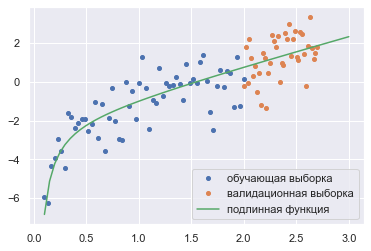
\includegraphics[width=\linewidth]{src/img/сгенерированная_выборка.png}
    \caption{Обучающая и валидационная выборки}
\end{wrapfigure}

Для заданной функции $f(h) = 1.5h - 2 - \frac{1}{2h}$ смоделируем обучающую выборку $f(h_k) + \varepsilon_k$. Точки $h_k$ выбраны равномерно на отрезке $[0.1;2]$, $к$ изменяется от $1$ до $60$. Аналогично смоделируем тестовую выборку с количеством наблюдений равным $40$. В качетсве параметров нормального распределения ошибок $\varepsilon$ было выбрано: $\mu=0, \sigma = 1$. Тестовая выборка была сгенерирована только по одну сторону от обучающей, поскольку заданная функция имеет полюс первого порядка в точке $h = 0$, и, следовательно функция при приближении к этой точке быстро растет, поэтому при генерировании точек вблизи $h=0$ значения могут быть крайне большими по модулю по сравнению с обучающей выборкой.
\newpage

\subsection{Метод наименьших квадратов}

Для модели простой линейной регрессии $X_k = \theta_0 + h\theta_1$ построим оценки МНК и МНМ, измерим качество, построенных моделей.

\begin{figure}[H]
    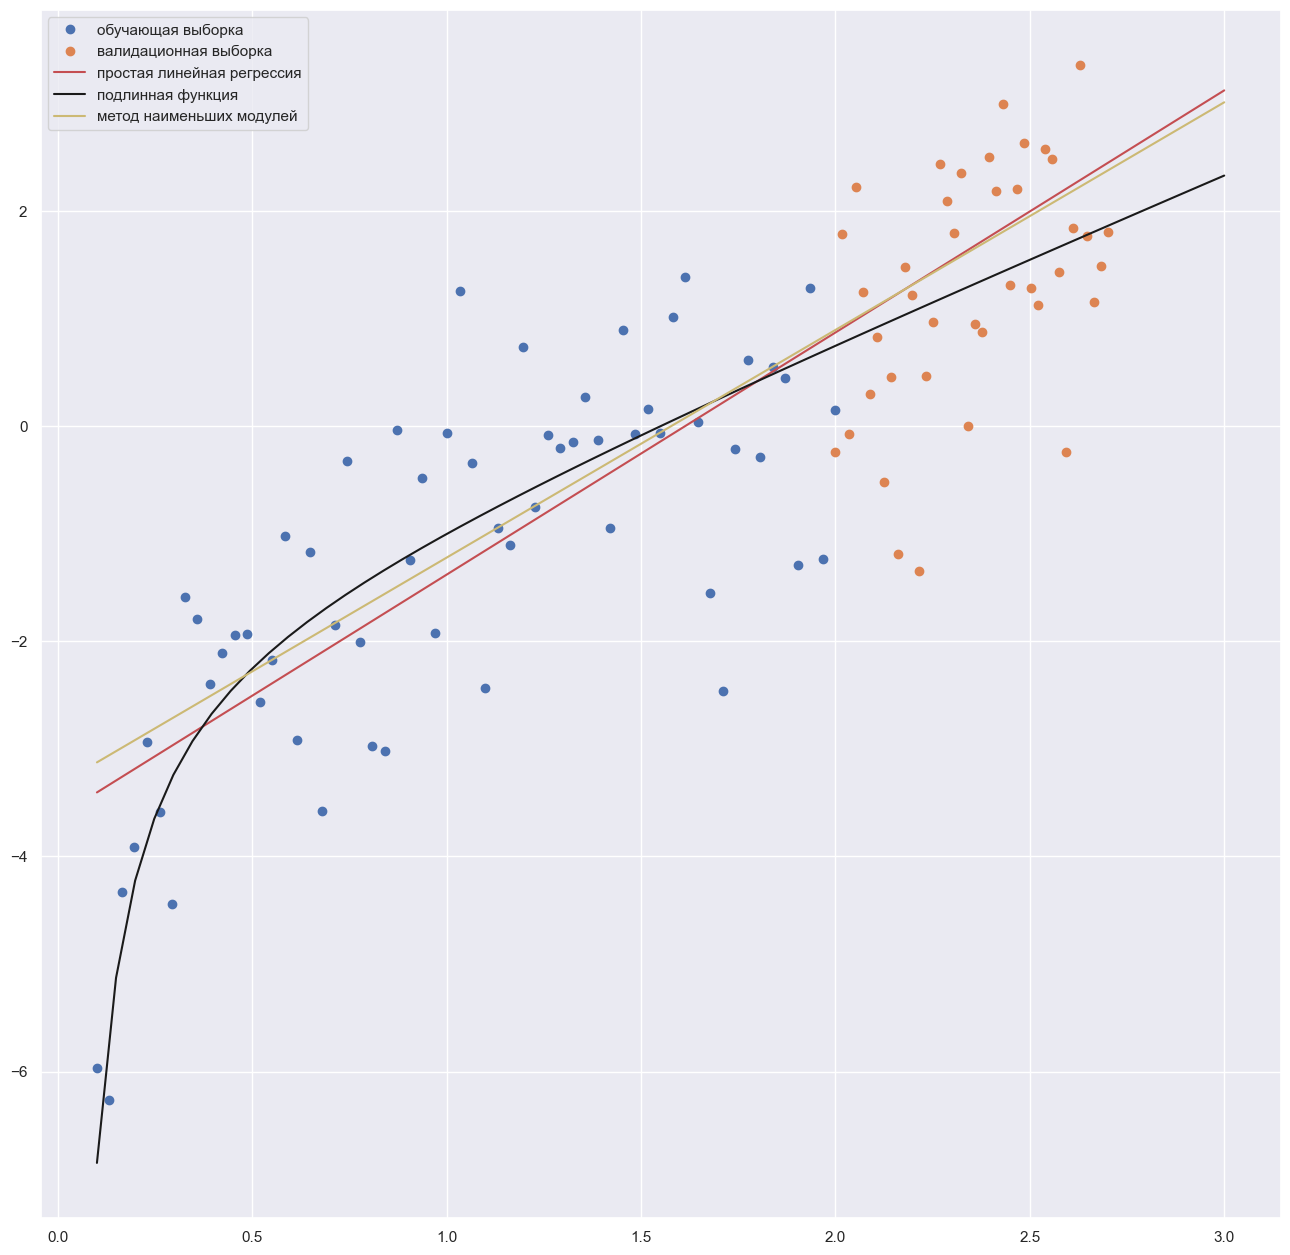
\includegraphics[width=\linewidth]{src/img/простая_линейная регрессия.png}
    \caption{Линии регрессии МНК и МНМ простой линейной регрессии}
\end{figure}

\begin{table}[H]
    \begin{center}
    \begin{tabular}{|l|c|c|}
        \hline
        & МНК & МНМ \\ \hline
        Уравнения прямых & $x = -3.63 + 2.25 h$ & $x = -3.34 + 2.12 h$ \\ \hline
        $R^2$ & $0.55$ & $0.55$ \\ \hline
        RMSE & $1.15$ & $1.16$ \\ \hline
        $\sum\limits_i \varepsilon_i^2$ (на обуч. выборке) & $78.87$ & $80.58$ \\ \hline
        $\sum\limits_i \varepsilon_i^2$ (на тест. выборке) & $44.22$ & $43.63$ \\ \hline
    \end{tabular}
    \caption{Сравнение моделей МНК и МНМ}
    \end{center}
\end{table}


\paragraph{Некоторые измерения модели с МНК.\\}

Оценка ковариационной матрицы:
$$ \hat{K} = 
\begin{pmatrix}
    0.10 & -0.08\\
    -0.08 & 0.08
\end{pmatrix}
$$
След оценки ковариационной матрицы $tr = 0.178$.

Функция логарифмического правдоподобия $l = -94.88$; информационный критерий Акаике $AIC = 0.39$; скорректированный (для малых выборок) $AIC_c = 0.6$; критерий Шварца $BIC = 197.95$.

Гипотеза, что $\forall i~\theta_i=0$ не принялась критерием Фишера на уровне значимости $\alpha = 0.05$.
Гипотеза, что $\theta_n = 0$ не принялась критерием Фишера на уровне значимости $\alpha = 0.05$.

Для проверки мультиколлинеарности матрицы $H^T H$ был использован коэффициент инфляции дисперсии (VIF).

Для данной модели $VIF = (4.54, 1.0)$, следовательно проблема мультиколлинеарности методом VIF не обнаружена.

\begin{figure}[H]
    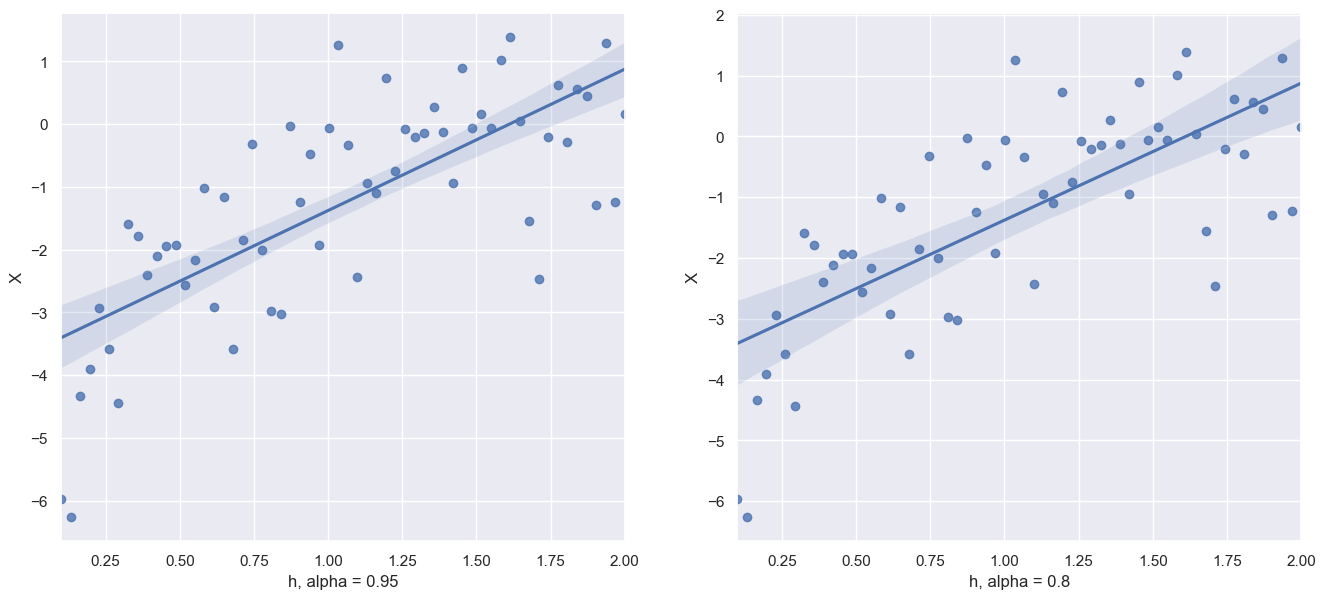
\includegraphics[width=\linewidth]{src/img/доврительные_интервалы.png}
    \caption{Доверительные интервалы для $X$ с надежностью 0.8 и 0.95}
\end{figure}


\paragraph{Анализ остатков.\\}
\begin{wrapfigure}{r}{0.3\linewidth}
    \vspace{-2ex}
    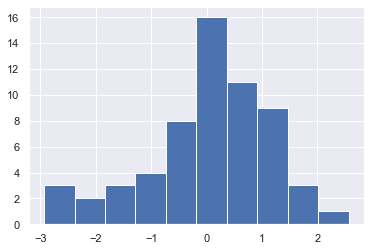
\includegraphics[width=\linewidth]{src/img/гистограмма_ошибок_1.png}
    \caption{Гистограмма ошибок}
\end{wrapfigure}

Критерий Шапиро-Уилка: $T = 0.98, pvalue = 0.29$.\\
Гипотезу о нормальном распределении ошибок на уровне значимости $0.05$ не удается принять.\\

Значение статистики Дарбина-Уотсона $ = 1.7$.\\
Выборочный коэффициент корреляции $r = 0.15$.\\
Гопотеза о некоррелированности принимается.\\

Критерий Бройша-Пагана: $(T_1 = 2.08, pvalue_1 = 0.15), (T_2 = 2.08, pvalue_2 = 0.15)$.\\
Гипотеза о гетероскедастичности принимается на уровне значимости $0.05$.\\

\begin{figure}[H]
    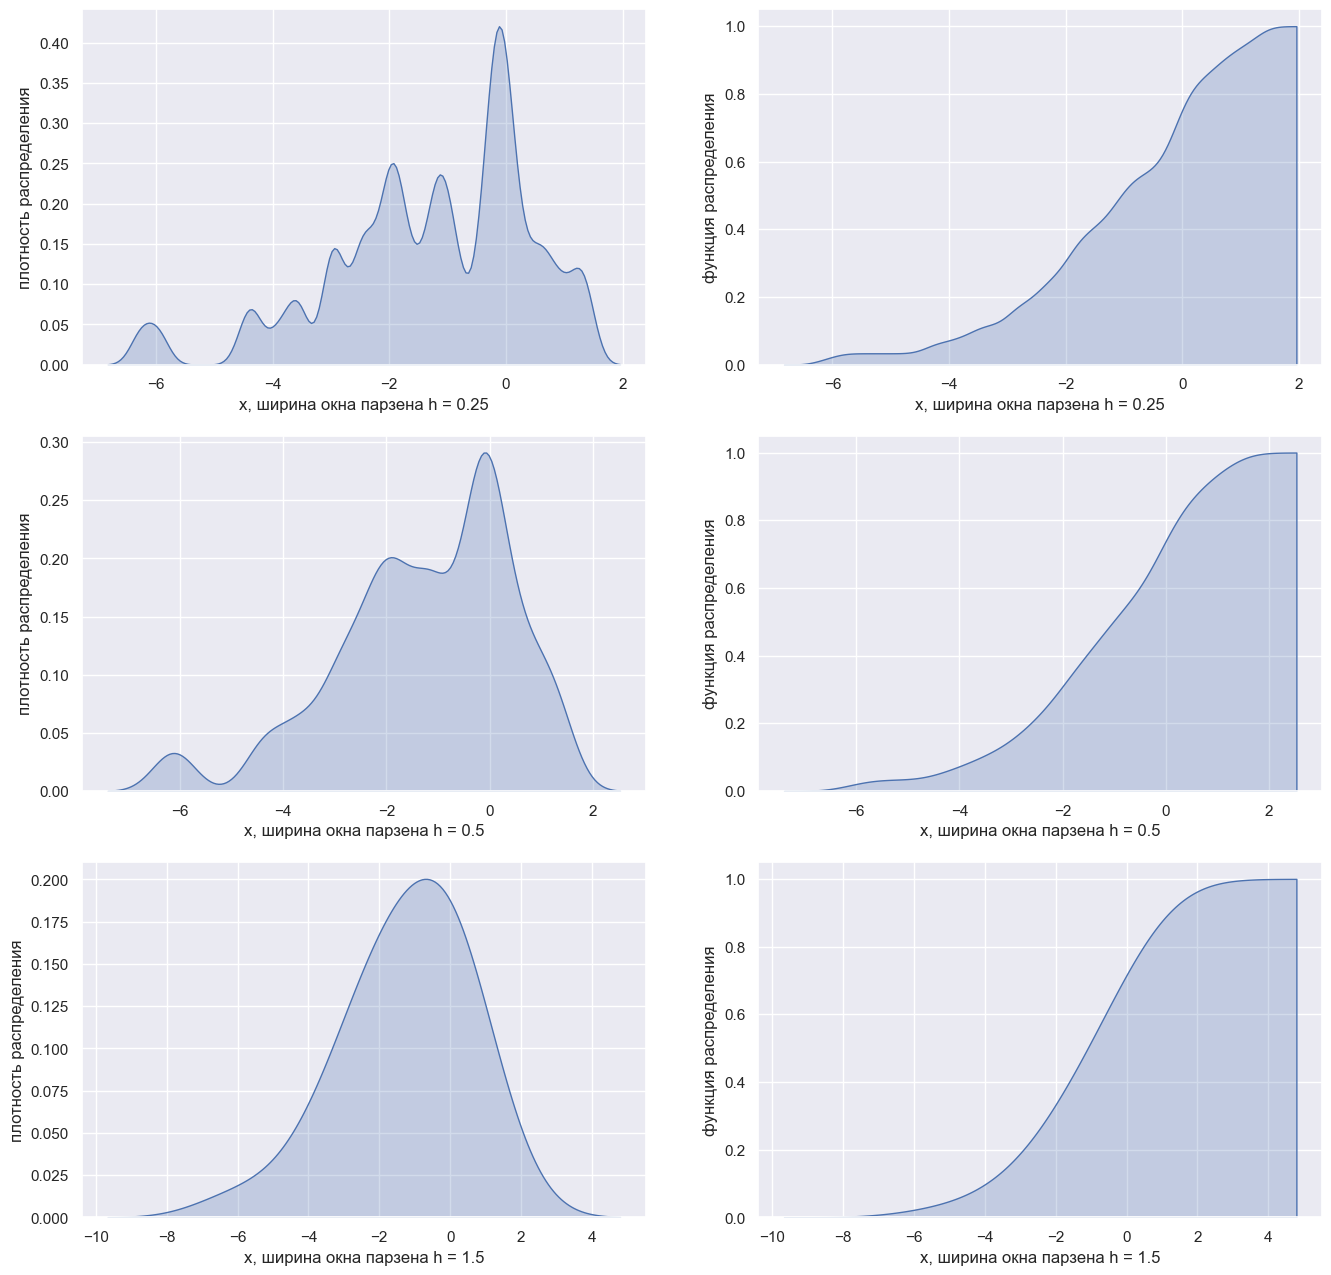
\includegraphics[width=\linewidth]{src/img/ядерные_оценки.png}
    \caption{Ядерные оценки плотности и распределения вероятности}
\end{figure}



\subsection{Полиномиальная регрессия}

\subsection{Регрессия для наблюдений с выбросами}

\subsection{Квантильная регрессия}



\section{Выводы}

\end{document}}